\documentclass[german,10pt]{book}      
\usepackage{makeidx}
\usepackage{babel}            % Sprachunterstuetzung
\usepackage{amsmath}          % AMS "Grundpaket"
\usepackage{amssymb,amsfonts,amsthm,amscd} 
\usepackage{mathrsfs}
\usepackage{rotating}
\usepackage{sidecap}
\usepackage{graphicx}
\usepackage{color}
\usepackage{fancybox}
\usepackage{tikz}
\usetikzlibrary{arrows,snakes,backgrounds}
\usepackage{hyperref}
\hypersetup{colorlinks=true,
                    linkcolor=blue,
                    filecolor=magenta,
                    urlcolor=cyan,
                    pdftitle={Overleaf Example},
                    pdfpagemode=FullScreen,}
%\newcommand{\hyperref}[1]{\ref{#1}}
%
\definecolor{Gray}{gray}{0.80}
\DeclareMathSymbol{,}{\mathord}{letters}{"3B}
%
\newcounter{num}
\renewcommand{\thenum}{\arabic{num}}
\newenvironment{anmerkungen}
   {\begin{list}{(\thenum)}{%
   \usecounter{num}%
   \leftmargin0pt
   \itemindent5pt
   \topsep0pt
   \labelwidth0pt}%
   }{\end{list}}
%
\renewcommand{\arraystretch}{1.15}                % in Formeln und Tabellen   
\renewcommand{\baselinestretch}{1.15}                 % 1.15 facher
                                                      % Zeilenabst.
\newcommand{\Anmerkung}[1]{{\begin{footnotesize}#1 \end{footnotesize}}\\[0.2cm]}
\newcommand{\comment}[1]{}
\setlength{\parindent}{0em}           % Nicht einruecken am Anfang der Zeile 

\setlength{\textwidth}{15.4cm}
\setlength{\textheight}{23.0cm}
\setlength{\oddsidemargin}{1.0mm} 
\setlength{\evensidemargin}{-6.5mm}
\setlength{\topmargin}{-10mm} 
\setlength{\headheight}{0mm}
\newcommand{\identity}{{\bf 1}}
%
\newcommand{\vs}{\vspace{0.3cm}}
\newcommand{\noi}{\noindent}
\newcommand{\leer}{}

\newcommand{\engl}[1]{[\textit{#1}]}
\parindent 1.2cm
\sloppy

         \begin{document}  \setcounter{chapter}{6}


\chapter{BB84 - Quantenkryptographie}
% Kap x
\label{chap_BB84}

\section*{Kurzzusammenfassung}

Eine gesicherte Nachrichten\"ubertragung ist mit einem Schl\"ussel m\"oglich, der
aus einer Zufallsfolge von Bits (0 und 1) besteht, der dieselbe L\"ange wie die zu
\"ubertragende Nachricht hat und der nur ein einziges Mal verwendet wird. Dieses
Protokoll bezeichnet man als One-Time Pad. Die meisten Verfahren der Quantenkryptographie, 
insbesondere auch das sogenannte BB84-Protokoll, verwenden die Quantentheorie
lediglich zur sicheren Erzeugung eines solchen Schl\"ussels (also einer Zufallsfolge
aus 0 und 1), von dem \"uberpr\"uft werden kann, dass nur der Sender und der
Empf\"anger diesen Schl\"ussel kennen. 

Eine wesentliche Eigenschaft der Quantentheorie, die dieses Verfahren erm\"oglicht,
ist das sogenannte \glqq No-Cloning\grqq-Theorem bzw.\ die Unm\"oglichkeit, einen
unbekannten Quantenzustand eines Systems durch die Messung an einem Einzelsystem
bestimmen zu k\"onnen. 

Alice erzeugt dazu eine Serie von Photonen, die sie in einer Zufallsfolge von 
horizontaler, vertikaler, $+45^\circ$-diagonaler und $-45^\circ$-diagonaler Polarisation 
pr\"apariert und an Bob versendet. Bob analysiert den Polarsationszustand dieser
Photonen mit Polarisationsstrahlteilern, deren Orientierung ebenfalls zuf\"allig auf
$h/v$ (horizontal/vertikal) oder $+/-$ ($+45^\circ$- und $-45^\circ$-diagonal) gestellt wird. 
Anschlie\ss end tauschen Alice und Bob \"uber einen klassischen Kanal
die Folge der Basissysteme ($h/v$ oder $+/-$) aus und
w\"ahlen nur die Ergebnisse, bei denen sie zuf\"allig dieselbe Basis gew\"ahlt haben.
Die dabei gemessenen Polarisationen definieren ihren Schl\"ussel. 

Eve kann die Photonen von Alice abfangen, \"ahnlich wie Bob die Polarisationszust\"ande
bez\"uglich zuf\"allig gew\"ahlter Basen untersuchen, und dann gezielt diese
Polarisationszust\"ande an Bob weiterleiten. In rund der H\"alfte der F\"alle wird ihre
Polarisation mit der von Alice \"ubereinstimmen und die Photonen wurden nicht ver\"andert.
In der H\"alfte der F\"alle w\"ahlt sie jedoch die falsche Polarisation, sodass Bob 
in diesen F\"allen wiederum in der H\"alfte der F\"alle ein anderes Ergebnis erh\"alt
als Alice (in der anderen H\"alfte der F\"alle sind die Ergebnisse zuf\"allig gleich). 
Durch einen Vergleich eines Teils ihres Schl\"ussels l\"asst sich diese
Diskrepanz nachweisen und somit feststellen, ob der Schl\"usselaustausch \glqq abgelauscht\grqq\
wurde.

\newpage

\section*{Einf\"uhrung}

Quantenkryptographie ist eine der vielen faszinierenden Anwendungen der Quanteninformation.
Die M\"oglichkeit, Nachrichten austauschen zu k\"onnen, ohne dass diese Nachrichten
von dritter Seite abgeh\"ort oder entschl\"usselt werden k\"onnen, bietet viele Anwendungen,
die - wie immer in solchen F\"allen - nat\"urlich auch missbraucht werden k\"onnen. 

Bei den meisten Protokollen zur Quantenkryptographie, unter anderem auch bei dem
Protokoll BB84 (benannt nach Charles Bennett und Gilles Brassard, die es 1984 entwickelten \cite{Bennett}), 
geht es allerdings nur darum, einen idealen Schl\"ussel - in diesem Fall eine Zufallsfolge von 
Bits - aus\-zu\-tauschen, der sp\"ater sowohl f\"ur die Verschl\"usselung als auch f\"ur die
Entschl\"usselung der Nachricht verwendet werden kann. Wichtig ist, dass man \"uberpr\"ufen kann, 
ob der Schl\"ussel au\ss er den beiden Teilnehmern (Sender und Empf\"anger der Nachricht) tats\"achlich 
niemandem bekannt ist. Genau das leistet das BB84 Protokoll. Die eigentliche Nachricht wird nach
klassischen Verfahren ver- und entschl\"usselt und auch in klassischer Form verschickt.

Um nicht immer von einer Senderin oder einem Sender $A$ und einer Senderin oder
einem Sender $B$ zu sprechen, haben sich in der Informationstheorie die Bezeichnungen 
\glqq Alice\grqq\ f\"ur die Senderin der
Nachricht und \glqq Bob\grqq\ f\"ur den Empf\"anger der Nachricht etabliert. Den Lauscher bzw.\ die
Lauscherin bezeichnet man meist als \glqq Eve\grqq, abgeleitet von der englischen Bezeichnung
\glqq evesdropper\grqq\ f\"ur Lauscher. 

F\"ur die \"Ubertragungssituation des BB84 Protokolls fordert man gewisse Bedingungen, die erf\"ullt
sein sollten, damit das Protokoll sicher ist. So haben sowohl Alice als auch Bob einen abgeschlossenen Bereich,
in den kein externer Lauscher eindringen kann. Ein Eingreifen von Eve ist nur w\"ahrend der
\"Ubertragung von Daten m\"oglich, solange sich diese Daten in einem offenen Bereich befinden. 
Au\ss erdem wird vorausgesetzt, dass sich Alice und Bob \"uber einen klassischen Kanal (z.B.\ Telefon
oder Videokanal) austauschen und dabei verifizieren k\"onnen, dass sie tats\"achlich mit
der jeweils anderen Person sprechen. Bei einem klassischen \"Ubertragungskanal wird also
angenommen, dass sich Eve nicht als Alice oder Bob ausgeben kann. In der Informatik bezeichnet man
diese Bedingung als Authentizit\"at. Allerdings kann Eve nat\"urlich einem solchen Gespr\"ach lauschen.

Wir beginnen mit einer kurzen Beschreibung des sogenannten One-Time-Pads, einem
Protokoll der klassischen Kryptographie, bei dem einmalig eine Zufallsfolge von
Bits sowohl vom Sender zur Verschl\"usselung als auch vom Empf\"anger der Nachricht zur
Entschl\"usselung verwendet wird. Anschlie\ss end wird beschrieben, wie man mit 
Verfahren der Quantentheorie einen solchen Schl\"ussel austauschen und gleichzeitig sicherstellen kann,
dass au\ss er Alice und Bob niemand den Schl\"ussel kennt.

\section{Klassische Kryptographie - das One-Time-Pad}

Ein One-Time-Pad ist spezielles Protokoll der klassischen Kryptographie, bei dem eine Nachricht
mit Hilfe einer Zufallsfolge von Bits vom Sender verschl\"usselt und vom Empf\"anger entschl\"usselt
werden kann. Sender und Empf\"anger m\"ussen diese Zufallsfolge kennen,
allerdings sollte niemand sonst Informationen \"uber diese Folge haben. Es gibt auch One-Time-Pads, bei denen dezimale 
Zahlenfolgen oder Buchstabenfolgen verwendet werden, doch sofern es
sich in allen F\"allen um wirkliche Zufallsfolgen handelt, sind
diese nicht sicherer als eine bin\"are Bitfolge. Man ben\"otigt allerdings bei
einer bin\"aren Nachrichten\"ubertragung mehr Zeichen. Au\ss erdem muss die zu verschl\"usselnde Nachricht
ebenfalls als Bitfolge vorliegen, was sich aber immer erreichen l\"asst. 
Der Schl\"ussel des One-Time-Pads sollte den folgenden vier Bedingungen
gen\"ugen:
\begin{enumerate}
\item
Die Bitfolge muss mindestens so lang sein wie der zu verschl\"usselnde Text.
\item
Es muss sich um eine Zufallsfolge von Bits handeln.
\item
Die Bitfolge oder Teile von ihr werden kein zweites Mal (weder in der vorliegenden Nachricht
noch in anderen Nachrichten) wiederverwendet. 
\item
Die Bitfolge darf nur dem Sender und dem Empf\"anger bekannt sein. Auch keine einschr\"ankenden 
Informationen \"uber die Bitfolge d\"urfen potenziellen Lauschern bekannt sein.
\end{enumerate}
Unter diesen Bedingungen kann man beweisen, dass eine entsprechend verschl\"usselte Nachricht
prinzipiell nicht entschl\"usselt werden kann. Der Grund ist
sehr einfach: Bei der mit einer Zufallsfolge verschl\"usselten Nachricht handelt es sich wieder
um eine Zufallsfolge, und wenn man alle m\"oglichen Schl\"ussel ausprobiert, erh\"alt man jede beliebige
Bitfolge und somit auch jeden beliebigen Text derselben L\"ange. Sofern \"uber den Schl\"ussel nichts
bekannt ist, kann man auch keine Information \"uber die urspr\"ungliche Nachricht gewinnen.   

Bedingung 1 und 3 lassen sich im Prinzip
sehr leicht erf\"ullen, sind aber in der Praxis oft ein Problem, da Sender
und Empf\"anger f\"ur den Bedarfsfall oft sehr lange Schl\"ussel austauschen oder vorr\"atig haben m\"ussen.  
Bedingung 2 ist etwas schwieriger, da die meisten
sogenannten Zufallszahlgeneratoren auf einem deterministischen Algorithmus beruhen und damit
f\"ur jemanden, der diesen Algorithmus sowie den Anfangszustand kennt, auch reproduzierbar sind. 
Die eigentliche Problematik ist aber Bedingung 4: Wie kann man sicher sein, dass niemand
au\ss er den Teilnehmern die Bitfolge kennt, insbesondere, wenn diese Bitfolge \"uber einen 
\"offentlichen bzw.\ abh\"orbaren Kanal ausgetauscht wurde? Wir werden sehen, dass sowohl Bedingung
2 als auch Bedingung 4 im Rahmen der Quantenkryptographie erf\"ullt werden k\"onnen. 

Ist eine Zufallsbitfolge gegeben, erfolgt die Verschl\"usselung durch eine XOR-Operation, also
eine Addition modulo 2, mit der zu verschl\"usselnden Nachricht. Die Rechenregeln sind:
\begin{equation}
     0+0=1+1=0 \hspace{1cm} 0+1=1+0=1 \, .
\end{equation} 
Die daraus entstandene Bitfolge ist unabh\"angig von der darin
enthaltenen Nachricht nach allen detektierbaren Kriterien ebenfalls wieder eine Zufallsfolge und kann
\"uber einen \"offentlichen Kanal verschickt werden. Der Empf\"anger kann diese verschl\"usselte Nachricht 
entziffern, indem er mit demselben Schl\"ussel nochmals eine XOR Operation durchf\"uhrt. Da sowohl
$0+0$ als auch $1+1$ bez\"uglich XOR die 0 ergeben, wird durch die insgesamt zweifache XOR
Addition des Schl\"ussels die urspr\"ungliche Nachricht wieder hergestellt. Dies zeigt folgendes Beispiel, bei dem
ein Klartext (abwechselnd dreimal 0 und dreimal 1)
mit einer Zufallsfolge zu einer verschl\"usselten Nachricht umgewandelt
und anschlie\ss end mit derselben Zufallsfolge wieder entschl\"usselt wird:
\begin{eqnarray}
\nonumber
  \mbox{Klartext} & &
  1~1~1~0~0~0~1~1~1~0~0~0~1~1~1~0~0~0~1~1~1~0~0~0 \\
  \nonumber
  \mbox{Zufallsfolge} & &
  0~1~1~0~1~0~0~0~1~0~1~1~1~0~1~1~0~1~0~0~1~0~0~1 \\
  \mbox{XOR-kodierte Nachricht} & &
  1~0~0~0~1~0~1~1~0~0~1~1~0~1~0~1~0~1~1~1~0~0~0~1 \\
\nonumber
  \mbox{Zufallsfolge} & &
  0~1~1~0~1~0~0~0~1~0~1~1~1~0~1~1~0~1~0~0~1~0~0~1 \\
\nonumber
 \mbox{XOR-Dekodierung=Klartext} & &
  1~1~1~0~0~0~1~1~1~0~0~0~1~1~1~0~0~0~1~1~1~0~0~0 
\end{eqnarray}

\section{Das BB84-Protokoll}

Wie schon erw\"ahnt geht es bei dem BB84-Protokoll nur um den sicheren Austausch eines
Schl\"ussels, also einer bin\"aren Zufallsfolge. Im Prinzip l\"asst sich das BB84-Protokoll mit jedem
QBit, also jedem quantenmechanischen Zwei-Zustandssystem durchf\"uhren, allerdings verwendet
man meist die linearen Polarisationszust\"ande von Photonen. 
F\"ur das BB84-Protokoll werden auch keine verschr\"ankten
Photonen ben\"otigt. Es gibt allerdings andere Protokolle, die von verschr\"ankten Zust\"anden
Gebrauch machen. 

\subsection{Messung und Pr\"aparation der Polarisation von Einzelphotonen}

Wichtig f\"ur das Verst\"andnis der Quantenkryptographie im Allgemeinen wie auch speziell
f\"ur dass BB84-Protokoll sind folgende Tatsachen:
\begin{enumerate}
\item
Ein unbekannter Polarisationszustand eines Einzelphotons kann nicht durch Messungen bestimmt werden. 
Ein polarisationsabh\"angiger Strahlteiler oder auch ein Polarisationsfilter hat immer eine
bestimmte Orientierung. Dadurch wird eine Basis aus zwei orthogonalen Polarisationszust\"anden 
ausgezeichnet. Eine \glqq Messung\grqq\ findet immer in Bezug auf diese Basis statt
und man erh\"alt einen der beiden m\"oglichen Basiszust\"ande als Ergebnis. 
Ob diese Polarisation auch vorher schon vorlag, ist dabei nicht bekannt. 
\item 
Quantenzust\"ande kann man nicht clonen, d.h., man kann keine Kopien
eines Quantenzustands herstellen und dabei das Original behalten. Die Quantenteleportation erlaubt
zwar die Erstellung einer Kopie, aber dabei geht das Original verloren, d.h., es gibt immer nur einen
Zustand mit den urspr\"unglichen Eigenschaften. 
\item Ist die Polarisationsbasis bekannt, d.h., ist bekannt,
bez\"uglich welcher Orientierung (z.B.\ eines Polarisationsstrahlteilers)
eine Polarisation pr\"apariert wurde, kann diese nat\"urlich auch
ausgelesen und kopiert werden. 
\end{enumerate}

Das Protokoll f\"ur den Schl\"usselaustausch besteht aus drei Schritten. In einem weiteren Schritt kann
\"uberpr\"uft werden, ob der Schl\"ussel abgeh\"ort wurde. Auf diesen letzten Schritt gehen wir in
Abschnitt \ref{sec_Test} ein, die ersten drei Schritte sind:
\begin{enumerate}
\item
Alice pr\"apariert zuf\"allig ausgew\"ahlte Polarisationszust\"ande von Photonen bez\"uglich 
zweier vorab festgelegter Orientierungen (Basissysteme) 
und verschickt diese an Bob. Diese Polarisationszust\"ande kodieren eine Bitfolge.
\item
Bob nimmt Polarisationsmessungen  an den Photonen vor, wobei er zwischen den beiden 
vorab festgelegten m\"oglichen Orientierungen (Basissystemen) zuf\"allig ausw\"ahlt. Er erh\"alt auf diese
Weise ebenfalls eine Bitfolge.
\item
Alice und Bob vergleichen \"uber einen klassischen Kanal, welche Basis sie bei den einzelnen Photonen
gew\"ahlt haben. Die Bitfolge in den \"ubereinstimmenden F\"allen ist ihre Zufallsfolge. 
\end{enumerate}
Diese Schritte werden im Folgenden eingehender behandelt.

\subsection{Alice pr\"apariert die Photonen f\"ur Bob}

Alice (die Senderin) m\"ochte sich mit  Bob (dem Empf\"anger) eine bin\"are Zufallsfolge teilen, die
nur sie beide kennen. Dazu ben\"ogt Alice zun\"achst eine Quelle von Einzelphotonen, denen 
sie gezielt bestimmte Polarisationszust\"ande verleihen kann. Sie w\"ahlt dabei zwischen vier m\"oglichen
Polarisationszust\"anden aus, die den Basiszust\"anden von zwei Orientierungen eines
Polarisationsstrahlteilers entsprechen: die Basiszust\"ande bez\"uglich
horizontaler-vertikaler Orientierung und die Basiszust\"ande bez\"uglich einer $+45^\circ$-$-45^\circ$ diagonalen
Orientierung (siehe Abb.\ \ref{fig_QKrypt}). Wenn im Folgenden von Orientierung die Rede ist, bezieht
sich dies immer auf die Wahl eines orthogonalen Basissystems. F\"ur jede Orientierung gibt es dann zwei
m\"ogliche Basiszust\"ande bzw.\ Polarisationszust\"ande.

\begin{SCfigure}[50][htb]
\begin{tikzpicture}
\draw (2,2) circle (1.5cm);
\draw (2,0.5) -- (2,3.5);
\draw (0.5,2) -- (3.5,2);
\draw (6,2) circle (1.5cm);
\draw (4.95,0.95) -- (7.05,3.05);
\draw (4.95,3.05) -- (7.05,0.95);
\draw (8,2) node{~};
\end{tikzpicture}
\caption{\label{fig_QKrypt}%
Die beiden Orientierungen bzw.\ 
Basissysteme f\"ur die Pr\"aparations- bzw.\ Mess\-an\-ordnungen beim BB84-Protokoll. 
(links) horizontal-vertikal ($h/v$-Basis), (rechts) $+45^\circ$-$-45^\circ$ ($+/-$-Basis).}
\end{SCfigure}

Alice erzeugt nun eine Folge von Einzelphotonen, die jeweils eine zuf\"allige Polarisation bez\"uglich
einer der beiden Polarisationsorientierungen haben, d.h.\ die zuf\"allig eine der vier Polarisationszust\"ande
$h$, $v$, $+$ oder $-$ haben. Das kann z.B.\ folgenderma\ss en geschehen (es geht
hier nur um ein Prinzip, nicht um die in der Praxis verwendete Realisierung): Es gibt nicht-lineare Kristalle
(z.B.\ Bariumborat, oft mit BBO abgek\"urzt), bei denen ein einfallendes 
Photon einer bestimmten Energie in zwei Photonen
von jeweils der halben Energie (doppelte Wellenl\"ange) umgewandelt wird. Eines dieser Photonen dient
als Signalphoton - es zeigt an, dass ein zweites Photon (das sogenannte Idler-Photon) in diesem Moment in eine 
bestimmte Richtung emittiert wird. Gew\"ohnlich hat dieses zweite Photon eine wohldefinierte
Polarisation, die Alice in eine der vier genannten Polarisationen drehen kann. Sie kennt also den genauen 
Polarisationszustand des Photons, das sie an Bob schickt. Alice sollte die Orientierungen, bez\"uglich der sie die 
Polarisationen pr\"apariert, zuf\"allig w\"ahlen.

Diese Folge von Einzelphotonen schickt Alice an Bob. Sie hat dabei f\"ur jedes einzelne dieser Photonen folgende
Information, die sie zun\"achst geheim h\"alt: Sie kennt die Basis, bez\"uglich der sie die Polarisation der Photonen
pr\"apariert hat, und sie kennt den zugeh\"origen Polarisationszustand dieses Photons. Hierbei verwendet man eine
Konvention, die vorher festgelegt wurde, z.B.\ $0$ f\"ur den Zustand $h$ in der $h/v$-Basis und $1$ 
f\"ur den Zustand $v$ in der $h/v$-Basis, entsprechend $0$ f\"ur den Zustand $+$ in der $+/-$-Basis und $1$ f\"ur
den Zustand $-$ in der $+/-$-Basis. Alice besitzt also eine
Tabelle wie in Tab.\ \ref{tab_Alice1}.
\begin{table}[htb]
\begin{tabular}{c|c|c|c|c|c|c|c|c|c|c|c|c|c}
Photon & 1 & 2 & 3 & 4 & 5 & 6 & 7 & 8 & 9 & 10 & 11 & 12 & 13  \\
Basis & $+/-$ & $+/-$ & $h/v$ & $+/-$ & $h/v$ & $h/v$ & $h/v$ & $+/-$ & $+/-$ & $h/v$ & $+/-$ & $+/-$  & $+/-$  \\
Zustand & $+$ & $-$ & $h$ & $+$ & $h$ & $h$ & $h$ & $-$ & $+$ & $h$ & $+$ & $+$ & $-$ \\
Bit & 1 & 0 & 0 & 1 & 0 & 0 & 0 & 0 & 1 & 0 & 1 & 1 & 0       
\end{tabular}
\caption{\label{tab_Alice1}%
Tabelle von Alice. Diese Tabelle enth\"alt die Polarisationszust\"ande der Photonen, die Alice an Bob verschickt.}         
\end{table}

\subsection{Bob nimmt an den Photonen von Alice Messungen vor}

Bob erh\"alt von Alice die Folge der Photonen und wei\ss\ nur, dass jedes einzelne Photon entweder bez\"uglich
der Basis $h/v$ oder bez\"uglich der Basis $+/-$ pr\"apariert wurde. Er nimmt nun an jedem dieser Photonen eine
Messung vor, wobei er die Basis dieser Messung, d.h.\ die Orientierung seines
Polarisationsstrahlteilers, ebenfalls zuf\"allig w\"ahlt. In ungef\"ahr der H\"alfte dieser Messungen
w\"ahlt Bob eine Basis, die mit der Pr\"aparationsbasis von Alice \"ubereinstimmt. In diesen F\"allen stimmt sein
Ergebnis mit dem Ergebnis von Alice \"uberein. In allen anderen F\"allen ist seine Basis von der
Pr\"aparationsbasis von Alice verschieden und seine Ergebnisse sind zuf\"allig. Bob erh\"alt dadurch eine 
\"ahnliche Tabelle wie vorher Alice (siehe Tab.\ \ref{tab_Bob1}). 
\begin{table}[htb]
\begin{tabular}{c|c|c|c|c|c|c|c|c|c|c|c|c|c}
Photon & 1 & \underline{2} & \underline{3} & 4 & 5 & 6 & \underline{7} & 8 & \underline{9} & 
                \underline{10} & 11 & 12 & \underline{13}  \\
Basis & $h/v$ & $+/-$ & $h/v$ & $h/v$ & $+/-$ & $+/-$ & $h/v$ & $h/v$ & $+/-$ & $h/v$ & $h/v$ & $h/v$ & $+/-$   \\
Zustand & $v$ & $-$ & $h$ & $h$ & $+$ & $-$ & $h$ & $h$ & $+$ & $h$ & $h$ & $v$ & $-$   \\
Bit & 1 & 0 & 0 & 0 & 1 & 0 & 0 & 0 & 1 & 0 & 0 & 1 & 0       
\end{tabular}
\caption{\label{tab_Bob1}%
Tabelle von Bob. Sie enth\"alt die Polarisationszust\"ande, die Bob an den Photonen von Alice gemessen hat. 
Stimmt die gew\"ahlte Basis mit der von Alice \"uberein (die Nummer der zugeh\"origen Photonen wurde
unterstrichen), sind die Ergebnisse gleich, andernfalls sind sie zuf\"allig.}         
\end{table}

\subsection{Alice und Bob vergleichen ihre Basissysteme}

Nachdem Alice ihre Photonen an Bob verschickt hat und Bob an diesen Photonen die genannten
Messungen vorgenommen hat, vergleichen Alice und Bob \"uber einen klassischen (offenen) Kanal die
Polari\-sations\-basen (also die Orientierungen), die sie jeweils f\"ur ihre Photonen bew\"ahlt haben.
In ungef\"ahr der H\"alfte der Photonen werden diese Orientierungen gleich sein. 

Dieser klassische Kanal kann ruhig abgeh\"ort werden: Die ausgetauschte Information ist nicht
mehr verwendbar, da Bob die Photonen schon vermessen hat und wegen des No-Cloning Theorems
auch beim Austausch der Photonen keine Kopien angefertigt werden konnten. Alice und Bob m\"ussen
nur sicherstellen, dass sie tats\"achlich miteinander kommunizieren und die ausgetauschte Information
authentisch \"ubertragen wird. 

Sie tauschen nat\"urlich nur die jeweils gew\"ahlen Basissysteme $h/v$ bzw.\ $+/-$ aus, keine
Informationen \"uber die dabei pr\"aparierten bzw.\ gemessenen Werte. Falls die Basis, die Alice zur
Pr\"aparation verwendet hat, und die Basis, in der Bob die Messung vorgenommen hat, dieselbe ist,
sollten die Werte \"ubereinstimmen. Alle anderen F\"alle werden verworfen, da in diesen F\"allen die
Bitwerte zuf\"allig gleich oder verschieden sein k\"onnen. 

Bob verschickt \"uber den klassischen Kanal im Wesentlichen die zweite Zeile seines Messprotokolls. 
Alice vergleicht diese Zeile mit ihrer zweiten Zeile und schickt an Bob die Nummern der Photonen zur\"uck,
f\"ur die beide Basen gleich sind. Das sind in obigem Fall die Photonen 2, 3, 7, 9, 10 und 13 (sie
wurden in Tabelle \ref{tab_Bob1} unterstrichen). 
Die Bit-Werte zu
diesen Photonen sind beiden bekannt und sie sind gleich. Haben Alice und Bob ihre Basen zuf\"allig
gew\"ahlt, handelt es sich auch um eine Zufallsfolge. Diese Folge k\"onnen sie als Schl\"ussel verwenden. 

\subsection{Eve}
\label{sec_Eve}

Da ein m\"oglicher Lauscher nur in die \"Ubertragung von Photonen oder von Information \"uber \"offentliche
Kan\"ale eingreifen kann, bleibt Eve nur eine M\"oglichkeit: Sie muss die Photonen, die Alice an Bob verschickt,
abfangen und ebenfalls Messungen an diesen Photonen vornehmen. Zu diesem Zeitpunkt ist noch nicht bekannt,
bez\"uglich welcher Basis Bob seine Photonen ausmessen wird, da er diese Photonen noch nicht
erhalten hat. Also w\"ahlt Eve zuf\"allig 
f\"ur jedes Photon eines der beiden Basissysteme. Auch sie erh\"alt so eine Folge von Bits sowie eine Tabelle
mit der von ihr gew\"ahlten Basis (siehe Tab.\ \ref{tab_Eve1}).    

\begin{table}[htb]
\begin{tabular}{c|c|c|c|c|c|c|c|c|c|c|c|c|c}
Photon & 1 & 2 & 3 & \underline{4} & \underline{5} & 6 & \underline{7} & 8 & 9 & 10 & 
                        \underline{11} & 12 & \underline{13}  \\
Basis & $h/v$ & $h/v$ & $+/-$ & $+/-$ & $h/v$ & $+/-$ & $h/v$ &$h/v$ &$h/v$ & $+/-$ & $+/-$ & $h/v$ & $+/-$ \\
Zustand & $v$ & $v$ & $-$ & $+$ & $h$ & $-$ & $h$ &$v$ &$h$ & $-$ & $+$ & $h$ & $-$ \\
Bit & 1 & 1 & 0 & 1 & 0 & 0 & 0 & 1 & 0 & 0 & 1 & 0 & 0       
\end{tabular}
\caption{\label{tab_Eve1}%
Tabelle von Eve der Photonenzust\"ande, die sie an den Photonen von Alice gemessen hat. Stimmt die Basis
mit der von Alice \"uberein, sind die Ergebnisse wieder gleich (unterstrichene Photonenzahlen). 
Sie schickt Photonen in den von ihr bestimmten Zust\"anden an Bob. Das ist das Beste, was sie unter diesen 
Umst\"anden machen kann. In rund der H\"alfte der F\"alle wird diese Basis mit der von Alice \"ubereinstimmen. In
den anderen F\"allen verschickt sie die Photonen in einem anderen Polarisationszustand.}         
\end{table}

In den obigen Tabellen hat Eve f\"ur die Photonen 4, 5, 7, 11 und 13 dieselbe Basis gew\"ahlt wie Alice. 
F\"ur die anderen Photonen sind ihre Ergebnisse zuf\"allig. Sie verschickt nun eine Folge von Photonen
an Bob, die exakt ihrer Tabelle entspricht, d.h., sowohl die Basissysteme sind f\"ur die einzelnen Photonen
dieselben als auch die Polarisationen, die sie in der jeweiligen Basis f\"ur die Photonen erhalten hat. 
Sie kann nur hoffen, dass m\"oglichst viele dieser Basissysteme mit den Basen von Alice \"ubereinstimmen. 

\subsection{\"Uberpr\"ufung der Zufallsfolge}
\label{sec_Test}

Der letzte Schritt, den Bob und Alice ausf\"uhren sollten, ist die \"Uberpr\"ufung, ob die ausgetauschten
Photonen abgefangen und durch Messungen manipuliert wurden. 
\begin{table}[htb]
\begin{tabular}{c|c|c|c|c|c|c|c|c|c|c|c|c|c}
{\small Photon} & 1 & 2 & 3 & 4 & 5 & 6 & 7 & 8 & 9 & 10 & 11 & 12 & 13  \\ \hline
{\small Alice Basis} & ${\scriptstyle +/-}$ & ${\scriptstyle +/-}$ & ${\scriptstyle h/v}$ & ${\scriptstyle +/-}$ & ${\scriptstyle h/v}$ & ${\scriptstyle h/v}$ 
          & ${\scriptstyle h/v}$ & ${\scriptstyle +/-}$ & ${\scriptstyle +/-}$ & ${\scriptstyle h/v}$ & ${\scriptstyle +/-}$ 
          & ${\scriptstyle +/-}$  & ${\scriptstyle +/-}$  \\
{\small Bit} & 1 & 0 & 0 & 1 & 0 & 0 & 0 & 0 & 1 & 0 & 1 & 1 & 0 \\ \hline      
{\small Bob Basis (oE)} & ${\scriptstyle h/v}$ & ${\scriptstyle +/-}$ & ${\scriptstyle h/v}$ & ${\scriptstyle h/v}$ & ${\scriptstyle +/-}$ & ${\scriptstyle +/-}$ 
          & ${\scriptstyle h/v}$ & ${\scriptstyle h/v}$ & ${\scriptstyle +/-}$ & ${\scriptstyle h/v}$ & ${\scriptstyle h/v}$ & ${\scriptstyle h/v}$ 
          & ${\scriptstyle +/-}$   \\
{\small Bit} & 1 & 0 & 0 & 0 & 1 & 0 & 0 & 0 & 1 & 0 & 0 & 1 & 0   \\    \hline
{\small Eve Basis}  & ${\scriptstyle h/v}$ & ${\scriptstyle h/v}$ & ${\scriptstyle +/-}$ & ${\scriptstyle +/-}$ & ${\scriptstyle h/v}$ & ${\scriptstyle +/-}$ 
         & ${\scriptstyle h/v}$ &${\scriptstyle h/v}$ &${\scriptstyle h/v}$ & ${\scriptstyle +/-}$ & ${\scriptstyle +/-}$ & ${\scriptstyle h/v}$ 
         & ${\scriptstyle +/-}$ \\
{\small Bit} & 1 & 1 & 0 & 1 & 0 & 0 & 0 & 1 & 0 & 0 & 1 & 0 & 0  \\ \hline     
{\small Bob Basis (mE)} & ${\scriptstyle h/v}$ & ${\scriptstyle +/-}$ & ${\scriptstyle h/v}$ & ${\scriptstyle h/v}$ & ${\scriptstyle +/-}$ 
         & ${\scriptstyle +/-}$ & ${\scriptstyle h/v}$ & ${\scriptstyle h/v}$ & ${\scriptstyle +/-}$ & ${\scriptstyle h/v}$ & ${\scriptstyle h/v}$ 
         & ${\scriptstyle h/v}$ & ${\scriptstyle +/-}$   \\
{\small Bit} & 1 & 1 & 0 & 0 & 1 & 0 & 0 & 1 & 1 & 1 & 0 & 0 & 0   \\    \hline
\end{tabular}
\caption{\label{tab_QKgesamt}%
Die gesamte Tabelle des BB84-Protokolls. Die erste Doppelzeile gibt die Basis und die Bits an, in
Bezug auf die Alice ihre Photonen pr\"apariert hat. Die n\"achste Doppelzeile entspricht dem, was Bob
f\"ur den Fall gemessen h\"atte, wenn Eve keine Photonen abgefangen h\"atte. Die dritte Doppelzeile zeigt die
Ergebnisse von Eve und die letzte Doppelzeile die Ergebnisse von Bob, die er erhalten hat, nachdem Eve
ihre Photonen so weitergeschickt hat, wie sie bei ihr gemessen wurden.}
\end{table}

Tabelle \ref{tab_QKgesamt} enth\"alt nochmals alle Resultate, die Alice, Bob und Eve erhalten haben, wobei bei
Bob unterschieden wird, ob er die Photonen direkt von Alice erhalten hat (oE - ohne Eve), oder ob
Eve die Photonen abgefangen und an ihnen Messungen vorgenommen hat (mE - mit Eve).

Nachdem Alice und Bob ihre Basissysteme ausgetauscht haben (dieses Gespr\"ach kann Eve abh\"oren,
sie kann zu diesem Zeitpunkt nicht mehr eingreifen) wissen sie, welche Bitfolge sie f\"ur ihren Schl\"ussel
nehmen k\"onnen. Zur \"Uberpr\"ufung verwenden sie nun eine ausreichende Anzahl dieser Bits und
vergleichen diese \"uber einen klassischen (offenen) Kanal. In der obigen Liste sind beispielsweise
Alice und Bob zu dem Schluss gekommen, dass sie bei den Photonen 2, 3, 7, 9, 10 und 13 dieselben
Werte haben sollten. Vergleichen sie nun diese Bits \"uber einen offenen Kanal stellen
sie fest, dass nach dem Eingriff von Eve Photon 2 und 10 nicht zu demselben Bit geh\"oren. Daraus
k\"onnen sie schlie\ss en, dass ihr Photonenaustausch abgefangen und manipuliert wurde. Sie werden
nun s\"amtliche Bits ihrer Folge verwerfen und einen neuen Schl\"usselaustausch versuchen. 

Alice und Bob sollten also deutlich mehr
Bits f\"ur ihren Schl\"ussel erstellen, als sie f\"ur die Verschl\"usselung ihrer Nachricht ben\"otigen. In der
Praxis kann man mehrere Tausend Bits des Schl\"ussels vergleichen und so ziemlich sicher feststellen,
ob der Schl\"ussel durch Eve manipuliert wurde. Eve hat, bei korrekter Durchf\"uhrung des Protokolls,
keine M\"oglichkeit, die fehlerhaften Bits zu unterdr\"ucken. 

Ganz grob kann man sagen, dass rund die H\"alfte der Bits, die Alice und Bob mit dem Verfahren
generieren, \"ubereinstimmen und f\"ur die Verschl\"usselung (bzw.\ einen Teil davon f\"ur den Test)
verwendet werden k\"onnen. Falls Eve die Photonen abgefangen und manipuliert hat, hat sie in rund
der H\"alfte dieser F\"alle eine andere Basis gew\"ahlt als Alice und Bob, und davon wird in rund
der H\"alfte der F\"alle das Bit bei Bob ein anderes sein als bei Alice. Ganz grob kann man also
sagen, dass ungef\"ahr
ein Viertel der Bits, die Alice und Bob als gemeinsame Folge identifiziert haben, bei einem
Eingriff von Eve andere Werte haben. Verwendet man einige Tausend Bits zur Verifikation des
Schl\"ussels, sollte ein solcher Eingriff auffallen. 

\section{Schulische Teilrealisierung durch Laserlicht}

Eine vollst\"andige Realisierung dieses Protokolls scheitert in der Schule schon an dem Problem,
dass kaum Experimente mit einzelnen Photonen m\"oglich sein werden. Man kann das Protokoll
aber teilweise realisieren, indem man Laserlicht mit Polarisationsfiltern pr\"apariert bzw.\ misst.
Die Zufallselemente, die bei Einzelphotonen bestimmen, welches Bit bei einer bestimmten Basis
gemessen wird, kann man durch einen W\"urfel ersetzen. Im Folgenden werden nochmals die
Schritte des Protokolls durchgespielt, wie man sie in der Schule mit einfachen Mitteln (Laserpointer,
Polarisationsfilter und geeigneten W\"urfeln) umsetzen kann. Die folgenden Schritte sollten 
ausreichend oft wiederholt werden. 

\begin{enumerate}
\item
Alice w\"urfelt f\"ur jedes \glqq Photon\grqq\ eine Basis. Bei einem normalen W\"urfel kann man
beispielsweise eine gerade Augenzahl f\"ur die Basis $h/v$ w\"ahlen und eine ungerade Augenzahl
f\"ur die Basis $+/-$. Es gibt aber auch W\"urfel, bei denen $h/v$ und $+/-$ schon auf den W\"urfelseiten
verteilt sind. Sie w\"urfelt ein zweites Mal und entscheidet damit, auf welche Polarisation der
Filter hinter ihrem Laser eingestellt wird (diese Polarisation sollte nat\"urlich mit der vorher
gew\"urfelten Basis vertr\"aglich sein). Dann sendet Alice an Bob Laserlicht, das der entsprechenden
Polarisation entspricht. 
\item
Bob entscheidet mit einem W\"urfel, bez\"uglich welcher Basis er das Laserlicht von Alice
messen m\"ochte. Er w\"ahlt nun diese Basis f\"ur die Polarisationsfilter, auf die er das Laserlicht
von Alice schickt. Bei manchen Aufbauten kann Alice ihr Laserlicht durch einen Strahlteiler
aufspalten und dann gleichzeitig auf die beiden orthogonal eingestellten Filter von Bob lenken.
Nun gibt es zwei M\"oglichkeiten: (1) Alice und Bob haben dieselbe Basis gew\"ahlt. Dann hat das
Laserlicht von Alice eine Polarisation, die nur von einem Filter bei Bob durchgelassen wird. 
Das zugeh\"orige Bit zu diesem Filter (sowie die gew\"ahlte Basis) vermerkt Bob in seiner Liste.
(2) Falls Bob eine andere Basis als Alice gew\"ahlt hat, erkennt er das daran, dass das Laserlicht von
Alice durch beide Filter hindurchgeht (und etwas abgeschw\"acht wird). 
In diesem Fall w\"urfelt er ein beliebiges Bit. Bei Einzelphotonen
w\"urde Bob in diesem Fall auch nur ein Ergebnis erhalten, d.h., er kann an diesem Punkt nicht
feststellen, dass er die falsche Basis gew\"ahlt hat. Das gew\"urfelte Bit
wird sp\"ater, nachdem die Basisstellungen ausgetauscht wurden, nicht gewertet, da sich dann
herausstellt, dass die Orientierungen verschieden gew\"ahlt waren. 
\item
Im letzten Schritt tauschen Bob und Alice ihre Basissysteme aus und sollten nun f\"ur die
F\"alle, in denen die Basis gleich war, dieselben Ergebnisse erhalten haben.
\item
Falls Eve in den Prozess eingeschaltet wird, macht sie folgende Schritte: Sie w\"urfelt eine Basis
und misst bez\"uglich dieser Basis die Polarisation des einfallenden Laserlichts. Stimmt ihre Basis
mit der von Alice \"uberein, misst sie nur hinter einem ihrer Filter Licht und vermerkt das entsprechende
Bit. Sind die Basen von Alice und Eve verschieden, beobachtet sie hinter beiden Filtern Laserlicht
und w\"urfelt ein Bit. Sie schickt nun Laserlicht
mit der Basis und Polarisation an Bob, die sie verwendet bzw.\ gemessen oder gew\"urfelt hat. 

Im Wesentlichen an diesem Punkt scheitert das Protokoll in der Realit\"at, wenn man tats\"achlich
mit Laserlicht statt mit Einzelphotonen arbeiten m\"ochte. Eve kann feststellen, ob sie dieselbe Basis
wie Alice gew\"ahlt hat oder nicht: Wenn Sie bei einer Basis hinter beiden Filtern Licht beobachtet, 
ist es die falsche Basis. Sie k\"onnte nun die richtige Basis w\"ahlen und die Photonen des Laserlichts mit der
richtigen Polarisation weiterleiten. Lauscht sie sp\"ater dem Vergleich der Basissysteme zwischen Alice und
Bob kann sie ebenfalls den Schl\"ussel ermitteln. Mit Einzelphotonen kann Eve die
richtige Basis nicht feststellen.
\item
Am Ende vergleichen Alice und Bob ihre Bits, von denen sie glauben, sie seien gleich.    
\end{enumerate}
Damit man ein Eingreifen von Eve bemerken kann, sollten insgesamt mindestens 15 bis 20 \glqq Photonen\grqq\
ausgetauscht werden. Das kann bei sorgf\"altiger Durchf\"uhrung des Experiments eine Weile dauern
(insbesondere, wenn man die Schritte von Eve ebenfalls durchf\"uhren m\"ochte), sodass leicht eine
Doppelstunde mit diesem Protokoll ben\"otigt wird. Andererseits macht es auch Spa\ss, wenn man
am Ende die Bits vergleicht und feststellt, ob bzw.\ dass Eve eingegriffen hat. Nach dem Austausch
von vier oder f\"unf \glqq Photonen\grqq\ kommt auch eine gewisse Routine hinzu und es geht schneller.
Au\ss erdem kann man auf diese Weise den Ablauf des Protokolls wirklich miterleben und begreifen.

\section{Fragen}

Dieser Abschnitt enth\"alt einige Fragen, die man zun\"achst selbst beantworten sollte.
Sie eignen sich auch f\"ur die Diskussion in der Schule.

\begin{enumerate}
\item
Weshalb sollte Bob die Orientierungen bei seinen Messungen zuf\"allig w\"ahlen?
Welche Gefahr besteht, wenn er f\"ur die Orientierungen beispielsweise abwechselnd
$h/v$ und $+/-$ w\"ahlt?

\solution{Die Gefahr besteht darin, dass Eve diese Vorliebe von Bob kennt. In diesem Fall w\"ahlt
sie dieselben Orientierungen bei den Messungen wie Bob. Wenn Alice und Bob sp\"ater ihre
gew\"ahlten Basissysteme vergleichen, erhalten sie dieselben \"Ubereinstimmungen wie Alice und
Eve. Bei den Photonen, bei denen die Orientierungen von Eve und Bob sich von denen von Alice
unterscheden, k\"onnen die Messwerte verschieden sein, doch diese Bits werden verworfen. Bei den
Bits, die behalten werden, stimmen Eve, Bob und Alice \"uberein. Alice und Bob werden also nicht
bemerken, dass sie belauscht wurden.}



\end{enumerate}


\begin{thebibliography}{99}
\bibitem{Bennett} Bennett, C.H., Brassard, G., \textit{Quantum cryptography: Public
        key distribution and coin tossing}; in \textit{Proceedings of IEEE International
        Conference on Computers, Systems and Signal Processing}, Vol.\ 175 (1984).       
\end{thebibliography}


\end{document}

